% Options for packages loaded elsewhere
\PassOptionsToPackage{unicode}{hyperref}
\PassOptionsToPackage{hyphens}{url}
\PassOptionsToPackage{dvipsnames,svgnames,x11names}{xcolor}
%
\documentclass[
  authoryear,
  preprint,
  3p]{elsarticle}

\usepackage{amsmath,amssymb}
\usepackage{iftex}
\ifPDFTeX
  \usepackage[T1]{fontenc}
  \usepackage[utf8]{inputenc}
  \usepackage{textcomp} % provide euro and other symbols
\else % if luatex or xetex
  \usepackage{unicode-math}
  \defaultfontfeatures{Scale=MatchLowercase}
  \defaultfontfeatures[\rmfamily]{Ligatures=TeX,Scale=1}
\fi
\usepackage{lmodern}
\ifPDFTeX\else  
    % xetex/luatex font selection
\fi
% Use upquote if available, for straight quotes in verbatim environments
\IfFileExists{upquote.sty}{\usepackage{upquote}}{}
\IfFileExists{microtype.sty}{% use microtype if available
  \usepackage[]{microtype}
  \UseMicrotypeSet[protrusion]{basicmath} % disable protrusion for tt fonts
}{}
\makeatletter
\@ifundefined{KOMAClassName}{% if non-KOMA class
  \IfFileExists{parskip.sty}{%
    \usepackage{parskip}
  }{% else
    \setlength{\parindent}{0pt}
    \setlength{\parskip}{6pt plus 2pt minus 1pt}}
}{% if KOMA class
  \KOMAoptions{parskip=half}}
\makeatother
\usepackage{xcolor}
\setlength{\emergencystretch}{3em} % prevent overfull lines
\setcounter{secnumdepth}{5}
% Make \paragraph and \subparagraph free-standing
\ifx\paragraph\undefined\else
  \let\oldparagraph\paragraph
  \renewcommand{\paragraph}[1]{\oldparagraph{#1}\mbox{}}
\fi
\ifx\subparagraph\undefined\else
  \let\oldsubparagraph\subparagraph
  \renewcommand{\subparagraph}[1]{\oldsubparagraph{#1}\mbox{}}
\fi


\providecommand{\tightlist}{%
  \setlength{\itemsep}{0pt}\setlength{\parskip}{0pt}}\usepackage{longtable,booktabs,array}
\usepackage{calc} % for calculating minipage widths
% Correct order of tables after \paragraph or \subparagraph
\usepackage{etoolbox}
\makeatletter
\patchcmd\longtable{\par}{\if@noskipsec\mbox{}\fi\par}{}{}
\makeatother
% Allow footnotes in longtable head/foot
\IfFileExists{footnotehyper.sty}{\usepackage{footnotehyper}}{\usepackage{footnote}}
\makesavenoteenv{longtable}
\usepackage{graphicx}
\makeatletter
\def\maxwidth{\ifdim\Gin@nat@width>\linewidth\linewidth\else\Gin@nat@width\fi}
\def\maxheight{\ifdim\Gin@nat@height>\textheight\textheight\else\Gin@nat@height\fi}
\makeatother
% Scale images if necessary, so that they will not overflow the page
% margins by default, and it is still possible to overwrite the defaults
% using explicit options in \includegraphics[width, height, ...]{}
\setkeys{Gin}{width=\maxwidth,height=\maxheight,keepaspectratio}
% Set default figure placement to htbp
\makeatletter
\def\fps@figure{htbp}
\makeatother

\makeatletter
\@ifpackageloaded{caption}{}{\usepackage{caption}}
\AtBeginDocument{%
\ifdefined\contentsname
  \renewcommand*\contentsname{Table of contents}
\else
  \newcommand\contentsname{Table of contents}
\fi
\ifdefined\listfigurename
  \renewcommand*\listfigurename{List of Figures}
\else
  \newcommand\listfigurename{List of Figures}
\fi
\ifdefined\listtablename
  \renewcommand*\listtablename{List of Tables}
\else
  \newcommand\listtablename{List of Tables}
\fi
\ifdefined\figurename
  \renewcommand*\figurename{Figure}
\else
  \newcommand\figurename{Figure}
\fi
\ifdefined\tablename
  \renewcommand*\tablename{Table}
\else
  \newcommand\tablename{Table}
\fi
}
\@ifpackageloaded{float}{}{\usepackage{float}}
\floatstyle{ruled}
\@ifundefined{c@chapter}{\newfloat{codelisting}{h}{lop}}{\newfloat{codelisting}{h}{lop}[chapter]}
\floatname{codelisting}{Listing}
\newcommand*\listoflistings{\listof{codelisting}{List of Listings}}
\makeatother
\makeatletter
\makeatother
\makeatletter
\@ifpackageloaded{caption}{}{\usepackage{caption}}
\@ifpackageloaded{subcaption}{}{\usepackage{subcaption}}
\makeatother
\journal{Journal of the Acoustical Society of America}
\ifLuaTeX
  \usepackage{selnolig}  % disable illegal ligatures
\fi
\usepackage[]{natbib}
\bibliographystyle{elsarticle-harv}
\usepackage{bookmark}

\IfFileExists{xurl.sty}{\usepackage{xurl}}{} % add URL line breaks if available
\urlstyle{same} % disable monospaced font for URLs
\hypersetup{
  pdftitle={SPI - Defining bespoke and archetypal context-dependent Soundscape Perception Indices},
  pdfauthor={Andrew Mitchell; Francesco Aletta; Tin Oberman; Jian Kang},
  pdfkeywords={keyword1, keyword2},
  colorlinks=true,
  linkcolor={blue},
  filecolor={Maroon},
  citecolor={Blue},
  urlcolor={Blue},
  pdfcreator={LaTeX via pandoc}}

\setlength{\parindent}{6pt}
\begin{document}

\begin{frontmatter}
\title{SPI - Defining bespoke and archetypal context-dependent
Soundscape Perception Indices}
\author[1]{Andrew Mitchell%
\corref{cor1}%
}
 \ead{andrew.mitchell.18@ucl.ac.uk} 
\author[1]{Francesco Aletta%
%
}
 \ead{f.aletta@ucl.ac.uk} 
\author[1]{Tin Oberman%
%
}
 \ead{t.oberman@ucl.ac.uk} 
\author[]{Jian Kang%
%
}
 \ead{j.kang@ucl.ac.uk} 

\affiliation[1]{organization={University College London, Institute for
Environmental Design \& Engineering},,postcodesep={}}

\cortext[cor1]{Corresponding author}




        
\begin{abstract}
The soundscape approach provides a basis for considering the holistic
perception of sound environments, in context. While steady advancements
have been made in methods for assessment and analysis, a gap exists for
comparing soundscapes and quantifying improvements in the
multi-dimensional perception of a soundscape. To this end, there is a
need for the creation of single value indices to compare soundscape
quality which incorporate context, aural diversity, and specific design
goals for a given application. Just as a variety of decibel-based
indices have been developed for various purposes (e.g.~\(L_{Aeq}\),
\(L_{Ceq}\), \(L_{90}\), \(L{den}\), etc.), the soundscape approach
requires the ability to create novel indices for different uses, but
which share a common language and understanding. We therefore propose a
unified framework for creating both bespoke and standardised single
index measures of soundscape perception based on the soundscape
circumplex model, allowing for new metrics to be defined in the future.
The implementation of this framework is demonstrated through the
creation of a public spaced typology-based index using data collected
under the SSID Protocol, which was designed specifically for the purpose
of defining soundscape indices. Indices developed under this framework
can enable a broader and more efficient application of the soundscape
approach.
\end{abstract}





\begin{keyword}
    keyword1 \sep 
    keyword2
\end{keyword}
\end{frontmatter}
    
\section{Introduction}\label{introduction}

The EU Green Paper on Future Noise Policy indicates that 80 million EU
citizens are suffering from unacceptable environmental noise levels,
according to the WHO recommendation \citep{Berglund1999Guidelines} and
the social cost of transport noise is 0.2-2\% of total GDP. The
publication of the EU Directive Relating to the Assessment and
Management of Environmental Noise (END)
\citep{EuropeanUnion2002Directive} in 2002 has led to major actions
across Europe, with reducing noise levels as the focus, for which
billions of Euros are being spent. However, it is widely recognised that
solely reducing sound level is not always feasible or cost-effective,
and more importantly, with only \textasciitilde30\% of environmental
noise annoyance depending on facets of parameters such as acoustic
energy \citep{Guski1997Psychological}, sound level reduction will not
necessarily lead to improved quality of life.

Soundscape design, separate from noise control engineering, is about the
relationships between human physiology, perception, the sound
environment, and its social/cultural context \citep{Kang2006Urban}.
Soundscape research represents a paradigm shift in that it combines
physical, social, and psychological approaches and considers
environmental sounds as a `resource' rather than `waste'
\citep{Kang2016Soundscape} relating to perceptual constructs rather than
just physical phenomena. However, the current research is still at the
stage of describing and identifying the problems and tends to be
fragmented and focussed on only special cases e.g.~subjective
evaluations of soundscapes for residential areas
\citep{SchulteFortkamp2013Introduction}. In the movement from noise
control to soundscape creation \citep{Aletta2015Soundscape}, a vital
step is the standardisation of methods to assess soundscape quality.

A common aim for implementing soundscape assessment in practice is to
compare the quality of different soundscapes. Often (but not always) the
goal is to identify a `good' soundscape compared to a `bad' soundscape.
However, this presents several challenges:

\begin{itemize}
\tightlist
\item
  What makes a soundscape good or bad is highly contextual;
\item
  On what metric should the quality rating be based?
\item
  How can we deal with different requirements and definitions of how a
  soundscape should be perceived?
\end{itemize}

In many cases, the ultimate aim is to be able to rank soundscapes based
on their quality. However, any ranking metric should be flexible and be
able to handle a variety of contexts and definitions of what a `good'
soundscape is for a given purpose. To address this, we will propose the
Soundscape Perception Index (SPI) framework, a flexible method for
defining single value indices of soundscape quality based on
distributions within the Soundscape Circumplex Model (SCM)
\citep[\citet{Axelsson2012Swedish},
\citet{Mitchell2022How}]{Axelsson2010principal}. This paper will
demonstrate the SPI framework and test whether it is capable of both
scoring soundscape quality and generating consistent rankings of
soundscapes across different contexts.

\subsection{Background}\label{background}

In \citet{Aletta2016Soundscape}, the authors defined a framework for
categorising the components of a soundscape assessment. They define
three aspects: soundscape descriptors, soundscape indicators, and
soundscape indices. Soundscape descriptors are defined as `measures of
how people perceive the acoustic environment' and soundscape indicators
as `measures used to predict the value of a soundscape descriptor'.
Soundscape indices can then be defined as `single value scales derived
from either descriptors or indicators that allow for comparison across
soundscapes' \citep{Kang2019Towards}. --\textgreater{}

Soundscape indicators refer to measurable aspects or attributes of a
soundscape, such as loudness, tonal characteristics, or spectral
content, which can be quantified through objective measurements or
signal processing techniques. In contrast, soundscape descriptors are
qualitative representations of the perceived characteristics of a
soundscape, often derived from listener evaluations, subjective
assessments, or semantic differential scales \citep{ISO12913Part2}.

Indices, the primary focus of this article, are single numerical values
that combine multiple indicators or descriptors to provide a
comprehensive representation of the overall soundscape perception. These
indices serve as powerful tools for quantifying and comparing
soundscapes, enabling decision-makers and stakeholders to assess the
impact of interventions, monitor changes over time, and prioritize areas
for improvement.

The Decibel (dB) is the earliest and most commonly used scientific index
measuring sound level. To represent the overall level of sound with a
single value on one scale, as the Decibel index does, is often
desirable. For this purpose, a number of different values representing
sounds at various frequencies must be combined. Several frequency
weighting networks have been developed since the 1930s, considering
typical human responses to sound based on equal-loudness-level contours
\citep{Fletcher1933Loudness} and, among them, the A-weighting network,
with resultant decibel values called dBA, has been commonly used in
almost all the national/international regulations
\citep{Kryter1970Effects}. However, there have been numerous criticisms
on its effectiveness \citep{Parmanen2007weighted} as the correlations
between dBA and perceived sound quality (e.g.~noise annoyance) are often
low \citep{Hellman1987Why}.

Another set of indices is psychoacoustic magnitudes, including loudness,
fluctuation strength or roughness, sharpness, and pitch strength,
development with sound quality studies of industrial products since the
1980's \citep{Zwicker2007Psychoacoustics}. These emerged when it was
conceived that acoustic emissions had further characteristics than just
level \citep{Blauert1997Sound}. But while psychoacoustic magnitudes have
been proved to be successful for the assessment of product sound
quality, in the field of environmental acoustics, their applicability
has been limited \citep{Fastl2006Psychoacoustic}, since a significant
feature of environmental acoustics is that there are multiple/dynamic
sound sources.

Attendant with the transition from a noise reduction to soundscape
paradigm is an urgent need for developing appropriate indices for
soundscape, rather than continuously using dBA
\citep{Andringa2013Positioning}.

\subsection{The need for Soundscape
Indices}\label{the-need-for-soundscape-indices}

Soundscape studies strive to understand the perception of a sound
environment, in context, including acoustic, (non-acoustic)
environmental, contextual, and personal factors. These factors combine
together to form a person's soundscape perception in complex interacting
ways \citep{Berglund2006Soundscape}. Humans and soundscapes have a
dynamic bidirectional relationship - while humans and their behaviour
directly influence their soundscape, humans and their behaviour are in
turn influenced by their soundscape
\citep{Erfanian2019Psychophysiological}.

When applied to urban sound and specifically to noise pollution, the
soundscape approach introduces three key considerations beyond
traditional noise control methods:

\begin{enumerate}
\def\labelenumi{\arabic{enumi}.}
\tightlist
\item
  considering all aspects of the environment which may influence
  perception, not just the sound level and spectral content;
\item
  an increased and integrated consideration of the varying impacts which
  different sound sources and sonic characteristics have on perception;
  and
\item
  a consideration of both the positive and negative dimensions of
  soundscape perception.
\end{enumerate}

This approach can enable better outcomes by identifying positive
soundscapes (in line with the END's mandate to `preserve environmental
noise quality where it is good' \citep{EuropeanUnion2002Directive}),
better identify specific sources of noise which impact soundscape
quality and pinpoint the characteristics which may need to be decreased,
and illuminate alternative methods which could be introduced to improve
a soundscape where a reduction of noise is impractical
\citep{Fiebig2018Does, Kang2018Impact}. These can all lead to more
opportunities to truly improve a space by identifying the causes of
positive soundscapes, while also potentially decreasing the costs of
noise mitigation by offering more targeted techniques and alternative
approaches.

The traditional focus on noise levels alone fails to capture the
complexity of soundscape perception, which encompasses a multitude of
factors beyond mere sound pressure levels. Factors such as the presence
of natural or human-made sounds, their temporal patterns, and the
overall contextual meaning ascribed to these sounds all contribute to
the holistic perception of a soundscape. Consequently, there is a
pressing need for the development of robust indices that can encapsulate
this multi-dimensional nature of soundscape perception, enabling
comparative evaluations and informing targeted interventions to enhance
the overall quality of acoustic environments \citep{Chen2023Developing}.

Across both the visual and the auditory domain, research has suggested
that a disconnect exists between the physical metrics used to describe
urban environments and how they are perceived
\citep{Kruize2019Exploring, Yang2005Acoustic}. In addition, this
disconnect can be extended further into how these environments influence
the health and well-being of their users. To gain a better understanding
of these spaces and their immpacts on people who work and live in
cities, we must create assessment methods and metrics which go beyond
merely characterising the physical environment and instead translate
through the user's perception \citep{Mitchell2022Predictive}.

\subsection{Motivations \& Goals}\label{motivations-goals}

The primary motivation behind the development of the Soundscape
Perception Indices (SPIs) framework stems from the need to address the
existing gap in quantifying and comparing soundscape quality across
diverse contexts and applications. By creating a unified framework for
defining these indices, the aim is to facilitate a broader and more
efficient application of the soundscape approach in various domains,
such as urban planning, environmental management, acoustic design, and
policy development.

The overarching aim of this framework is to empower stakeholders,
decision-makers, and researchers with the ability to create tailored
indices that align with their specific objectives and design goals,
while simultaneously enabling cross-comparisons and benchmarking against
empirically-defined soundscape archetypes. This dual approach not only
acknowledges the context-dependent nature of soundscape perception but
also fosters a common language and understanding, facilitating knowledge
sharing and collaborative efforts within the field.

\emph{Ranking} - The ability to rank soundscapes based on their quality
is a key goal of the SPI framework. This ranking can be used to compare
soundscapes across different contexts, identify areas for improvement,
and prioritize interventions accordingly.

\emph{Standardisation} - The SPI framework aims to provide a
standardized approach for defining and calculating soundscape indices,
ensuring consistency and comparability across different applications and
domains. This standardization enables the development of best practices
and facilitates knowledge exchange within the field.

\section{Methodology}\label{methodology}

An index framework called the Soundscape Perception Indices (SPI) is
defined here as the agreement between an observed or modelled soundscape
perception distribution and a target soundscape perception distribution.
We refer to this as an index framework rather than a single index, as
the SPI can be tailored to specific contexts and applications by
defining a range of target distributions. A single index is thus created
for each target distribution, Throughout this manuscript we will discuss
several methods of applications for SPI indices.

\subsection{Dataset}\label{dataset}

We use the data contained in the International Soundscape Database (ISD)
(Mitchell et al., 2021a), which includes 1300+ individual responses
collected across 13 locations in London and Venice, according to the
SSID Protocol \citet{Mitchell2020Soundscape}.

\subsection{Soundscape Circumplex \&
Projection}\label{soundscape-circumplex-projection}

SPI is grounded in the soundscape circumplex model
\citep{Axelsson2010principal, Axelsson2012Swedish}, a robust theoretical
foundation for understanding and representing the multi-dimensional
nature of soundscape perception. The reason for grounding the SPI in the
soundscape circumplex is that we have observed this model (and its
corresponding PAQs) to become the most prevalent assessment model in
soundscape literature \citep{Aletta2023Adoption}.

Method A is built on a series of descriptors referred to as the
Perceived Affective Quality (PAQ), proposed by
\citep{Axelsson2010principal}. These PAQs are based on the
pleasantness-activity paradigm present in research on emotions and
environmental psychology, in particular Russell's circumplex model of
affect \citep{Russell1980circumplex}. As summarised by Axelsson:
``Russell's model identifies two dimensions related to the perceived
pleasantness of environments and how activating or arousing the
environment is.''

One benefit of the circumplex model is that, as a whole, it encapsulates
several of the other proposed soundscape descriptors - in particular,
annoyance, pleasantness, tranquility, and possibly restorativeness
\citep{Aletta2016Soundscape}. According to \citet{Axelsson2015How}, the
two-dimensional circumplex model of perceived affective quality provides
the most comprehensive information for soundscape assessment. It is also
possible that the overall soundscape quality could itself be derived
from the pleasant-eventful scores derived for a soundscape. The
circumplex also lends itself well to questionnaire-based methods of data
collection, as proposed in \citet{ISO12913Part2}. In contrast to methods
such as soundwalks, interviews, and lab experiments, in-situ
questionnaires are able to provide the quality and amount of data which
is necessary for statistical modelling. Combined, these factors make the
circumplex most appropriate for a single index as it provides a
comprehensive summary of soundscape perception.

To move the 8-item PAQ responses into the 2-dimensional circumplex
space, we use the projection method first presented in ISO 12913-3:2018.
This projection method and its associated formulae were recently updated
further in \citet{Mitchell2023Testing} to include a correction for the
language in which the survey was conducted. The formulae are as follows:

\[
P_{ISO} = \frac{1}{\lambda_{Pl}} \sum_{i=1}^{8} \cos \theta_i \cdot \sigma_i
\]

\[
E_{ISO} = \frac{1}{\lambda_{Ev}} \sum_{i=1}^{8} \sin \theta_i \cdot \sigma_i 
\]

Revise

\[
\lambda_{Pl} = \frac{\rho}{2} \sum_{i=1}^{8} |\cos \theta_i|
\]

\[
\lambda_{Ev} = \frac{\rho}{2} \sum_{i=1}^{8} |\sin \theta_i|
\]

Using the angles derived in \citet{Mitchell2023Testing}, the following
table is used to convert the angles into the ISO 12913-3:2018 circumplex
space:

\begin{longtable}[]{@{}lllllllll@{}}

\caption{\label{tbl-lang-angles}Language-specific angles for projection
into the ISO 12913-3:2018 circumplex space.}

\tabularnewline

\toprule\noalign{}
& PAQ1 & PAQ2 & PAQ3 & PAQ4 & PAQ5 & PAQ6 & PAQ7 & PAQ8 \\
\midrule\noalign{}
\endhead
\bottomrule\noalign{}
\endlastfoot
eng & 0 & 46 & 94 & 138 & 177 & 241 & 275 & 340 \\
arb & 0 & 36 & 45 & 135 & 167 & 201 & 242 & 308 \\
cmn & 0 & 18 & 38 & 154 & 171 & 196 & 217 & 318 \\
hrv & 0 & 84 & 93 & 160 & 173 & 243 & 273 & 354 \\
nld & 0 & 43 & 111 & 125 & 174 & 257 & 307 & 341 \\
deu & 0 & 64 & 97 & 132 & 182 & 254 & 282 & 336 \\
ell & 0 & 72 & 86 & 133 & 161 & 233 & 267 & 328 \\
ind & 0 & 53 & 104 & 123 & 139 & 202 & 284 & 308 \\
ita & 0 & 57 & 104 & 143 & 170 & 274 & 285 & 336 \\
spa & 0 & 41 & 103 & 147 & 174 & 238 & 279 & 332 \\
swe & 0 & 66 & 87 & 146 & 175 & 249 & 275 & 335 \\
tur & 0 & 55 & 97 & 106 & 157 & 254 & 289 & 313 \\

\end{longtable}

\textsubscript{Source:
\href{https://MitchellAcoustics.github.io/J2401_JASA_SSID-Single-Index/notebooks/SingleIndex-Code.ipynb.html\#cell-tbl-lang-angles}{SPI
- Defining bespoke and archetypal context-dependent Soundscape
Perception Indices}}

\subsection{Circumplex Distribution}\label{sec-circumplex-distribution}

Once the individual perceptual responses are projected into the
circumplex space, the resulting data for each location is treated as a
circumplex distribution. The circumplex is defined by two axes:
\(P_{ISO}\) and \(E_{ISO}\), which are limited to the range
\([-1, +1]\). Typically, data in the soundscape circumplex is treated as
a combination of two independent normal distributions, one for each axis
\citep{Mitchell2022How}. In some applications, this approach is
sufficient for capturing the distribution of soundscape perception,
however the method for calculating the SPI requires a more precise
approach. The independent normal distribution approach relies on three
key assumptions:

\begin{enumerate}
\def\labelenumi{\arabic{enumi}.}
\tightlist
\item
  The two axes are normally distributed.
\item
  The two axes are independent of each other.
\item
  The two axes are symmetrically distributed.
\end{enumerate}

While the first assumption is generally valid, the second and third
assumptions are not always met in practice. In particular, the
distribution of soundscape perception responses in the circumplex is
often characterised by a high degree of skewness, which can lead to
inaccuracies in the calculation of the SPI. Soundscape circumplex
distributions are most appropriately described as a bivariate
skew-normal distribution \citep{Azzalini2005Skew} which accurately
reflects the relationship between the two dimensions of the circumplex
and the fact that real-world perceptual distributions have been
consistently observed to not be strictly symmetric.

The skew-normal distribution is defined by three parameters: location
(\(\mu\)), scale (\(\sigma\)), and shape (\(\alpha\)). The location
parameter defines the centre of the distribution, the scale parameter
defines the spread of the distribution and the shape parameter defines
the skew of the distribution. The one-dimensional skew-normal
distribution is defined as \citep{Azzalini1996Multivariate}:

\[
\phi(z; \alpha) = 2 \phi(z) \Phi(\alpha z) \quad \text{for} \quad z \in \mathbb{R}
\]

where \(\phi\) and \(\Phi\) are the standard normal probability density
function and distribution function, respectively, and \(\alpha\) is a
shape variable which regulates the skewness. The distribution reduces to
a standard normal density when \(\alpha = 0\). The bivariate skew-normal
distribution extends this concept to two dimensions, allowing for the
modelling of asymmetric and skewed distributions in a two-dimensional
space such as the soundscape circumplex. The multivariate skew-normal
(MSN) distribution including scale and location parameters is given by
combining the normal density and distribution functions
\citep{Azzalini1999Statistical}:

\[
Y = 2 \phi_k (y-\xi; \Omega) \Phi\{\alpha^T\omega^{-1}(y-\xi)\} 
\]

where \(\phi_k\) is the \emph{k}-dimensional normal density with
location \(\xi\), shape \(\alpha\), and covariance matrix \(\Omega\).
\(\Phi \{ \dot \}\) is the normal distribution function and \(\alpha\)
is a \emph{k}-dimensional shape vector. When \(\alpha = 0\), \(Y\)
reduces to the standard multivariate normal \(N_k(\xi, \Omega)\)
density. A circumplex distribution can therefore be parameterised with a
2x2 covariance matrix \(\Omega\), a 2x1 location vector \(\xi\), and a
2x1 shape vector \(\alpha\), written as:

\[
Y \sim MSN (\xi, \Omega, \alpha)
\]

By fitting an MSN distribution to the soundscape perception responses,
it becomes possible to accurately capture the asymmetry and skewness of
the distribution. A bivariate skew-normal distribution can be summarised
as a set of these three parameters. Once parameterised, the distribution
can then be sampled from to generate a synthetic distribution of
soundscape perception responses. A demonstration of the results of this
process is shown in Figure~\ref{fig-dist-example} using data from a
single location included in the ISD.

\begin{figure}[H]

\centering{

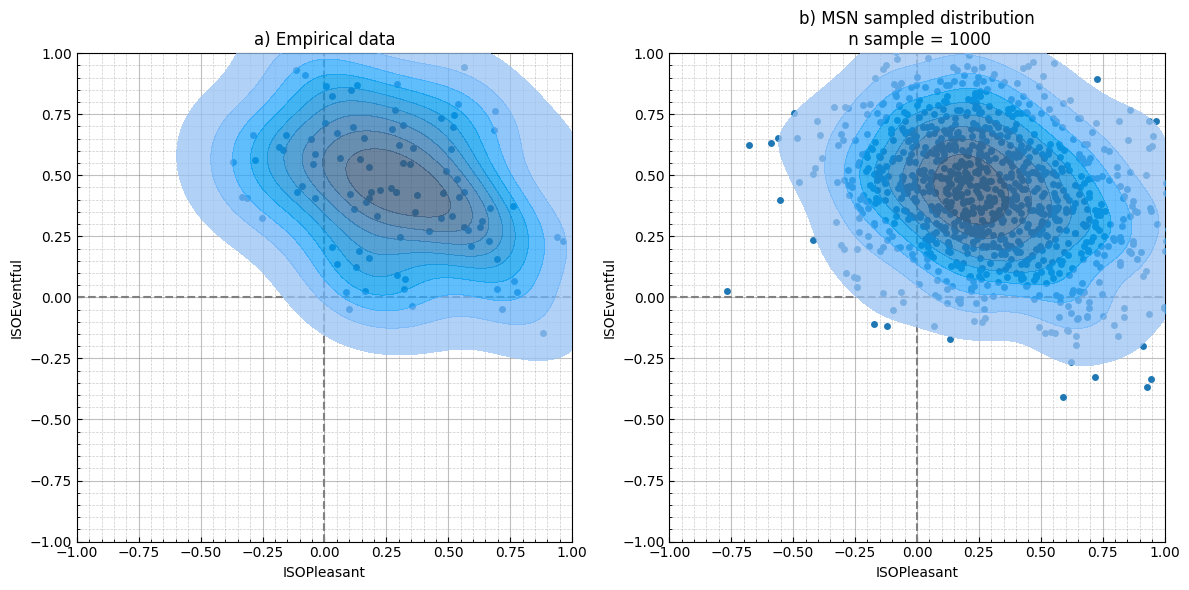
\includegraphics{index_files/figure-latex/notebooks-SingleIndex-Code-fig-dist-example-output-1.png}

}

\caption{\label{fig-dist-example}Example of fitting and sampling from a
multivariate skew-normal distribution for data from the Piazza San Marco
location.}

\end{figure}%

\textsubscript{Source:
\href{https://MitchellAcoustics.github.io/J2401_JASA_SSID-Single-Index/notebooks/SingleIndex-Code.ipynb.html\#cell-fig-dist-example}{SPI
- Defining bespoke and archetypal context-dependent Soundscape
Perception Indices}}

The parameters for the distribution shown in
Figure~\ref{fig-dist-example} are given by:

\[
MSN([0.065, 0.679], \begin{bmatrix} 0.149 & -0.064 \\ -0.064 & 0.101 \end{bmatrix}, [0.791, -0.767])
\]

\subsection{Defining the SPI
Framework}\label{defining-the-spi-framework}

The Soundscape Perception Indices (SPI) framework is centred around the
concept of quantifying the distance between a test distribution of
interest and the desired target distribution. Its goal is to determine
whether a soundscape - whether it be a real-world location, a proposed
design, or a hypothetical scenario - aligns with the desired perception
of that soundscape. This is achieved by first defining the target
distribution, which could represent what is considered to be the `ideal'
soundscape perception for a given context or application. The test
distribution is then compared to the target distribution using a
distance metric, which quantifies the deviation between the two
distributions. The resulting distance value serves as the basis for
calculating the SPI, with smaller distances indicating a closer
alignment between the perceived soundscape and the target soundscape
perception.

Although it is expected that the target distribution would usually
represent the ideal or goal soundscape perception, it is also possible
to define target distributions that represent undesirable or suboptimal
soundscape perceptions. For instance, in a soundscape mapping context,
it may be beneficial to map and identify chaotic soundscapes across a
city in order to better target areas for soundscape interventions. In
this case, the target distribution would be set in the chaotic quadrant
and a higher SPI would indicate a closer alignment with the target
distribution. This flexibility allows the SPI to be applied to a wide
range of contexts and applications, enabling the quantification and
comparison of soundscape quality across diverse scenarios.

An SPI value therefore does not represent a `good' or `bad' soundscape,
but rather a measure of how closely the perceived soundscape aligns with
the desired target soundscape perception. This approach allows for the
development of bespoke indices tailored to specific design goals and
objectives, while also enabling cross-comparisons and benchmarking
against empirically-defined soundscape archetypes.

\subsubsection{Defining a Target}\label{defining-a-target}

As introduced in Section~\ref{sec-circumplex-distribution}, circumplex
data follows a bivariate skew-normal distribution which can be
parameterised with a set of direct parameters (dp). We therefore define
a target distribution as a set of these parameters, which can then be
used to generate a synthetic distribution of soundscape perception
responses.

\subsubsection{Distance Metric}\label{distance-metric}

Central to the SPI framework is the concept of a distance metric, which
quantifies the deviation of a given soundscape from a desired target
soundscape. This distance metric serves as the basis for calculating the
SPI value, with smaller distances indicating a closer alignment between
the perceived soundscape and the target soundscape perception. The
distance between the test and target soundscape distributions is
calculated using a two-dimensional Kolmogorov-Smirnov test
\citep{Fasano1987multidimensional}.

Essentially, we approach this as a problem of (dis)similarity between
soundscapes. The distance metric is then proposed to assess how similar
two any given soundscapes distributions are within the circumplex. Taken
to the extreme, two perfectly matching distributions in the soundscape
circumplex would return a 100\% SPI value, while two completely
dissimilar distributions would return a 0\% SPI value. In practical
terms, for the former, this will never be achieved in real world
scenarios; for the latter, it is also difficult to estimate how low the
SPI value could actually go, and it should be considered that the
distance may happen in different directions within the circumplex space.
For instance, if a distribution for a vibrant soundscape was taken as a
reference, a compared soundscape distribution may exhibit low SPI values
for being located in the calm, OR monotonous, OR chaotic regions of the
model.

\subsubsection{Targets}\label{targets}

The SPI framework introduces two distinct types of targets: bespoke
targets and archetypal targets, each serving a unique purpose in the
index development process.

\paragraph{Bespoke Targets}\label{bespoke-targets}

Bespoke targets are tailor-made for specific projects, reflecting the
desired soundscape perception for a particular application. These
targets can be defined by stakeholders, designers, policymakers, or
decision-makers based on their unique requirements, objectives, and
constraints. This flexibility allows the SPI for a specific project to
be tailored to the desire of the stakeholders for how that specific
soundscape should function. It can also provide a consistent and
quantifiable baseline for scenarios like a soundscape design contest
wherein a target is specified and provided to all participants in the
contest and the winning proposal is the design with the highest SPI
score when assessed against that target.

\paragraph{Archetypal Targets}\label{archetypal-targets}

In contrast to bespoke targets, archetypal targets represent
generalized, widely recognized soundscape archetypes which transcend
specific applications or projects. These archetypes serve as reference
points and enable comparisons across different domains and use cases.
\textbf{\emph{By providing a framework for these archetypes to be
defined, they can be\ldots{}}}

Additionally, archetypal SPIs can be composed of multiple targets.

\subsubsection{Data Source}\label{data-source}

The SPI framework is designed to accommodate a wide range of data
sources, including both objective measurements and subjective
evaluations. This flexibility enables the framework to be applied to
diverse contexts and applications, ranging from urban soundscapes to
natural environments, public spaces, and indoor settings.

\subsection{Deriving a target}\label{deriving-a-target}


  \bibliography{FellowshipRefs-biblatex.bib}


\end{document}
